\documentclass[mat1, tisk]{fmfdelo}
% \documentclass[fin1, tisk]{fmfdelo}
% Če pobrišete možnost tisk, bodo povezave obarvane,
% na začetku pa ne bo praznih strani po naslovu, …

%%%%%%%%%%%%%%%%%%%%%%%%%%%%%%%%%%%%%%%%%%%%%%%%%%%%%%%%%%%%%%%%%%%%%%%%%%%%%%%
% METAPODATKI
%%%%%%%%%%%%%%%%%%%%%%%%%%%%%%%%%%%%%%%%%%%%%%%%%%%%%%%%%%%%%%%%%%%%%%%%%%%%%%%

% - vaše ime
\avtor{Tjaž Eržen}

% - naslov dela v slovenščini
\naslov{Paralelizacija grafovskih algoritmov v funkcijskih programskih jezikih}

% - naslov dela v angleščini
\title{Parallelisation of Graph Algorithms in Functional Programming Languages}

% - ime mentorja/mentorice s polnim nazivom:
\mentor{doc.~dr.~Matija Pretnar}

% - leto diplome
\letnica{2024} 



% - povzetek v slovenščini
%   V povzetku na kratko opišite vsebinske rezultate dela. Sem ne sodi razlaga
%   organizacije dela, torej v katerem razdelku je kaj, pač pa le opis vsebine.
\povzetek{
Diplomska naloga obravnava paralelizacijo grafovskih algoritmov v funkcijskih programskih jezikih, s poudarkom na OCamlu in uporabi knjižnice Domainslib.
Delo se osredotoča na razvoj in analizo paralelnih različic klasičnih algoritmov, kot so iskanje v širino (BFS), Dijkstrov algoritem in Floyd-Warshallov algoritem.
Glavni cilj je bil primerjati učinkovitost paralelnih in sekvenčnih implementacij teh algoritmov v kontekstu funkcijskega programiranja.
Analiza je pokazala, da paralelna implementacija lahko izboljša učinkovitost, še posebej pri obsežnih grafih, čeprav je izbor optimalnega števila procesorskih domen ključnega
pomena za maksimalno zmogljivost.
}

% - povzetek v angleščini
\abstract{
This thesis addresses the parallelization of graph algorithms in functional programming languages, with a focus on OCaml and the use of the Domainslib library.
The work concentrates on developing and analyzing parallel versions of classical algorithms, such as breadth-first search (BFS), Dijkstra's algorithm, and the Floyd-Warshall algorithm.
The primary goal was to compare the effectiveness of parallel and sequential implementations of these algorithms in the context of functional programming.

The analysis showed that parallel implementation can improve efficiency, especially in extensive graphs, although the choice of the optimal number of processor domains is crucial for maximum performance.
}

% - klasifikacijske oznake, ločene z vejicami
%   Oznake, ki opisujejo področje dela, so dostopne na strani https://www.ams.org/msc/
\klasifikacija{68R10, 68W10, 68N18, 68N19, 05C85}

% - ključne besede, ki nastopajo v delu, ločene s \sep
\kljucnebesede{paralelizacija\sep grafovski algoritmi\sep funkcijski programski jeziki\sep OCaml\sep iskanje v širino (BFS)\sep Dijkstrov algoritem\sep Floyd-Warshallov algoritem\sep večjedrno računanje}

% - angleški prevod ključnih besed
\keywords{parallelisation\sep graph algorithms\sep functional programming languages\sep OCaml\sep breadth-first search (BFS)\sep Dijkstra's algorithm\sep Floyd-Warshall algorithm\sep multi-core computing}

% - angleško-slovenski slovar strokovnih izrazov
\slovar{
  \geslo{paralelizacija}{parallelization}
  \geslo{grafovski algoritmi}{graph algorithms}
  \geslo{funkcijski programski jeziki}{functional programming languages}
  \geslo{OCaml}{OCaml}
  \geslo{iskanje v širino (BFS)}{breadth-first search (BFS)}
  \geslo{Dijkstrov algoritem}{Dijkstra's algorithm}
  \geslo{Floyd-Warshallov algoritem}{Floyd-Warshall algorithm}
  \geslo{Domainslib}{Domainslib}
  \geslo{nespremenljive podatkovne strukture}{immutable data structures}
  \geslo{večjedrno računanje}{multi-core computing}
  \geslo{optimizacija algoritmov}{algorithm optimization}
  \geslo{dinamično programiranje}{dynamic programming}
  \geslo{vrsta s prednostjo}{priority queue}
  \geslo{računska učinkovitost}{computational efficiency}
  \geslo{visokonivojske abstrakcije}{high-level abstractions}
}

% - ime datoteke z viri (vključno s končnico .bib), če uporabljate BibTeX

\literatura{literatura.bib}


%%%%%%%%%%%%%%%%%%%%%%%%%%%%%%%%%%%%%%%%%%%%%%%%%%%%%%%%%%%%%%%%%%%%%%%%%%%%%%%
% DODATNE DEFINICIJE
%%%%%%%%%%%%%%%%%%%%%%%%%%%%%%%%%%%%%%%%%%%%%%%%%%%%%%%%%%%%%%%%%%%%%%%%%%%%%%%

% naložite dodatne pakete, ki jih potrebujete
\usepackage{algpseudocode}  % za psevdokodo
\usepackage{algorithm}      % za algoritme
\usepackage{algorithmicx}
\usepackage{hyperref}
\usepackage{listings}
\usepackage{tikz}
\usepackage{circuitikz}
\usetikzlibrary{shapes,arrows}

\hypersetup{
    colorlinks=true,
    linkcolor=blue,
    filecolor=magenta,
    urlcolor=cyan,
    citecolor=red
}

% Set the font size for all listings
\lstset{basicstyle=\footnotesize\ttfamily}

\algnewcommand\algorithmicto{\textbf{to}}
\algnewcommand\algorithmicin{\textbf{in}}
\algnewcommand\algorithmicforeach{\textbf{for each}}
\algrenewtext{For}[3]{\algorithmicfor\ #1 $\gets$ #2\ \algorithmicto\ #3\ \algorithmicdo}
\algdef{S}[FOR]{ForEach}[2]{\algorithmicforeach\ #1\ \algorithmicin\ #2\ \algorithmicdo}


\floatname{algorithm}{Algoritem}
\renewcommand{\listalgorithmname}{Kazalo algoritmov}

\newcommand{\R}{\mathbb R}
\newcommand{\N}{\mathbb N}
\newcommand{\Z}{\mathbb Z}
\newcommand{\C}{\mathbb C}
\newcommand{\Q}{\mathbb Q}

\lstdefinelanguage{OCaml}{
  keywords={let,rec,if,then,else,module},
  sensitive=true,
  basicstyle=\ttfamily,
  keywordstyle=\bfseries,
  showstringspaces=false,
  morecomment=[s]{(*}{*)},
  morestring=[b]"
}

\lstset{
  language=Caml,
  frame=single,
  numbers=left,
  numberstyle=\tiny,
  stepnumber=1,
  numbersep=5pt,
  tabsize=2,
  breaklines=true,
  prebreak=\raisebox{0ex}[0ex][0ex]{\ensuremath{\hookleftarrow}},
  showtabs=false,
  showspaces=false,
  showstringspaces=false,
  basicstyle=\ttfamily\small,
  identifierstyle=\ttfamily\small,
  commentstyle=\color{gray}\ttfamily\small,
  keywordstyle=\color{blue}\ttfamily\small,
  stringstyle=\color{red}\ttfamily\small
}


%%%%%%%%%%%%%%%%%%%%%%%%%%%%%%%%%%%%%%%%%%%%%%%%%%%%%%%%%%%%%%%%%%%%%%%%%%%%%%%
% ZAČETEK VSEBINE
%%%%%%%%%%%%%%%%%%%%%%%%%%%%%%%%%%%%%%%%%%%%%%%%%%%%%%%%%%%%%%%%%%%%%%%%%%%%%%%

\begin{document}

\section{Uvod}

Grafovski algoritmi so ključni pri modeliranju širokega nabora vsakdanjih problemov.
Igrajo pomembno vlogo pri modeliranju družbenih ter računalniških omrežjih, z njimi pa se prav tako razrešujejo 
problemi na področjih računalniške komunikacije in podatkovne analitike. Splošno, z grafi  modeliramo kakršne 
koli odnose med danimi entitetami, vse od računanja razdalj med mesti, pa do računanje vodnega pretoka
od enega kraja do drugega.

Z večanjem kompleksnosti grafov naraščajo tudi zahteve za računsko moč pri njihovem obdelovanju.
Načinov za reševanje tega problema je več, pogosto pa je eden izmed možnih načinov pospešitve programa paralelizacija,
s čimer bolje izkoristimo celotno računsko kapaciteto računalnika. Posledično je paralelizacija tovrstnih algoritmov
v zadnjih letih postala tako zanimiva raziskovalna kot tudi aplikativna tema v računalništvu.

Vzporednost na nivoju procesorja je moč doseči na dva načina: 
Tako, da je pomnilnik vsem računalniškim jedrom \textit{skupen}, ali pa da je pomnilnik \textit{porazdeljen}. 
V tej diplomski nalogi se bomo posvetili zgolj sistemom s skupnim pomnilnikom ter porazdeljeno procesorsko močjo, 
saj je tovrstne programe tipično manj zahtevno implementirati, kot pa tiste, ki delujejo na porazdeljenem pomnilniku.

Vse več funkcijskih programskih jezikov, kot so na primer Scala, Haskell in OCaml ima implementirane knjižnice
in ogrodja za paralelizacijo grafovskih algoritmov:
\begin{itemize}
    \item knjižnica \textit{fgl} v Haskellu \cite{haskell_fgl} zagotavlja vzporedne algoritme za najkrajšo pot 
    ter iskanje krepko povezanih komponent,
    \item \textit{GraphX} v Scali \cite{graphx} ponuja implementacijo paralelnega Googlovega PageRank algoritma,
    \item \textit{Ocaml 500} v OCamlu \cite{ocaml_multicore_500} ponuja implementacijo paralelnega iskanja v širino ter paralelnega Dijkstrovega algoritma na redkih grafih.
\end{itemize}

Z izdajo različice 5.0.0 je leta 2022 programski jezik OCaml pridobil podporo za paralelno računanje.
V tej diplomski nalogi bomo raziskali implementacijo paralelnih grafovskih algoritmov v OCamlu, s
poudarkom na uporabi knjižnice Domainslib. Implementirane bodo paralelne različice klasičnih algoritmov, kot so
iskanje v širino (BFS), Dijkstrov algoritem in Floyd-Warshallov algoritem.

Zaradi relativno nedavne uvedbe podpore za paralelizacijo v OCamlu, je literature na temo paralelnega programiranja v OCamlu
omejeno. Ta omejitev je spodbudila k uporabi OCamlove dokumentacije o paralelizaciji \cite{ocaml_paralelisation_documentation}
in raziskovanju metod in knjižnic, razvitih za druge funkcijske jezike. Konkretno, za razvoj struktur grafov je bila uporabljena knjižnica,
razvita v Swiftu \cite{functional_swift_graph}, medtem ko so za implementacijo grafovskih algoritmov in oblikovanje knjižnice uporabljene
tehnike iz Haskellove knjižnice fgl \cite{haskell_fgl}. Med obstoječimi viri v OCamlu je bila kot osrednji vir uporabljena knjižnica
OCaml 500 \cite{ocaml_multicore_500}, ki je bila ključna za razumevanje in izvajanje paralelne obdelave.

\subsection{Kaj lahko od paralelnega programa pričakujemo?}

V praksi se od paralelnega programa običajno pričakuje višja hitrost izvajanja v primerjavi s sekvenčnim programom,
kjer se naloge izvajajo zaporedno. Teoretično lahko pričakujemo, da program, ki deluje na $n$ procesorjih,
doseže do $n$-krat večjo hitrost, vendar je ključno upoštevati dodatne računske obremenitve, ki nastanejo pri vzpostavitvi
paralelnega izvajanja. Te obremenitve vključujejo sinhronizacijo procesov, upravljanje virov in koordinacijo med procesorskimi enotami.
Zaradi teh dejavnikov lahko paralelni program v nekaterih primerih, še posebej pri izvajanju na enem samem jedru,
postane počasnejši od sekvenčnega ekvivalenta. Ta pojav poudarja pomembnost razmisleka o optimalnem razporejanju
nalog in upravljanju virov, da se maksimizira izkoristek paralelizacije. Slika \ref{fig:cilj-casovne-zahtevnosti-paralelizacije} prikazuje
naša pričakovanja od paralelnega programa.

\begin{figure}[h!]
  \centering
  \caption{V našem programu si želimo, da bo čas izvedbe našega programa ujet med spodnjo in zgornjo mejo.}
  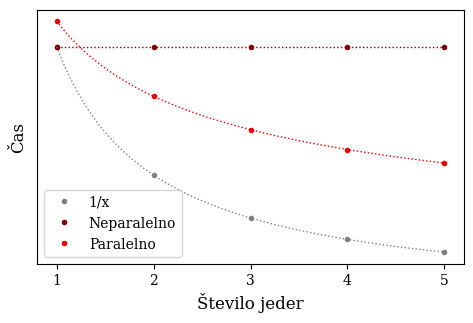
\includegraphics[width=13cm]{slike/cilj-casovne-zahtevnosti-paralelizacije.png}
  \label{fig:cilj-casovne-zahtevnosti-paralelizacije}
\end{figure}

\subsection{Prednosti paralelizacije v funkcijskih programskih jezikih}

\emph{Stranski učinki} so v programiranju kakršen koli odklon med čistimi matematičnimi funkcijami ter našim programom.

Zakaj koncepta funkcijskih programskih jezikov ter paralelizacije tako dobro sovpadata skupaj?
V primerjavi z drugimi vrstami programskih jezikov, kot so na primer imperativni programski jeziki,
so funkcijski programski jeziki bolj primerni za paralelizacijo iz več razlogov 
\cite{linke_fundamental_2015, functional_parallel_graph_rewriting}:

\begin{itemize} \label{itemize:prednosti_funkcijskega_programiranja}
  \item \textbf{Nespremenljivost in odsotnost stranskih učinkov:} 
    Elementarne podatkovne strukture v funkcijskih programskih jezikih so običajno nespremenljive, kar za sabo prinese številne
    prednosti, kot so na primer lažje razumevanje, enostavnejše odpravljanje napak ter boljša modularnost.
    Vse te lastnosti pa so še posebej pomembne v paralelnem kontekstu, kjer so naloge pogosto razdeljene med
    različne niti. Če nam je zagotovljeno, da naša funkcija ne spreminja nobenega skupnega stanja, se
    različni procesi lahko izvajajo vzporedno, ne da bi se pri tem bilo treba ukvarjati s tem, da bi več procesov
    naenkrat posegalo po istem prostoru v pomnilniku, ali z drugimi sinhronizacijskimi težavami.
    Iz praktičnih izkušenj je razvidno, da uporaba spremenljivih podatkovnih struktur v OCamlu, kot sta na primer
    \texttt{Array} in \texttt{reference}, lahko povzroči težave pri pisanju paralelnih programov, saj to zahteva
    dodatno usklajevanje stanja med procesi.

  \item \textbf{Lažje razumevanje in odpravljanje napak:} 
    Odsotnost stranskih učinkov prav tako olajša razumevanje kode in odpravljanje napak., kar je še posebej
    pomembno pri paralelnem programiranju, kjer je težko slediti stanju programa.

  \item \textbf{Modularnost in ponovna uporabnost:}
    Funkcijsko programiranje spodbuja pisanje majhnih, čistih funkcij, s čimer poskrbimo, da je naša koda bolj 
    modularna in ponovno uporabna. To je lahko velika prednost v paralelnem kontekstu,
    kjer je naloge pogosto treba razbiti na manjše, neodvisne enote, ki se lahko izvajajo vzporedno.

  \item \textbf{Deklarativna narava funkcijskih jezikov:} 
    Funkcijsko programiranje je oblika deklarativnega programiranja, kar pomeni, da opišemo, kaj želimo doseči, 
    ne da bi natančno opisali, kako to doseči. Ta visoka stopnja abstrakcije lahko olajša pisanje paralelne kode, 
    saj se lahko osredotočite na problem, ne da bi se zapletli v podrobnosti paralelnega izvajanja.
\end{itemize}

Ko potrebujemo implementacijo določene podatkovne strukture v imperativnem programskem jeziku, kot je na primer
\textit{Python}, je pogosto dovolj, da v splošnem učbeniku najdemo njeno implementacijo ter jo prepišemo.
Razvijalci, ki pa svojo kodo pišejo v funkcijskih programskih jezikih, pa zaradi manjše
razširjenosti funkcijskih programskih jezikov pogosto te sreče nimajo.
Dodatno smo zaradi stroge omejitve odsotnosti stranskih učinkov v funkcijskih jezikih primorani, da se izogibamo
programskim konstruktom, ki pomnilnik spreminjajo, na primer zanka. To pa je v primeru implementacije grafovskih
algoritmov, kjer se moramo npr. sprehoditi po sosedih trenutnega vozlišča, pogosto precej težavno.

Obstajajo primeri, ko podatkovna struktura, uporabljena v imperativnih jezikih, nima neposrednega ekvivalenta v funkcijskih jezikih.
Pri implementaciji različnih podatkovnih struktur, kot je na primer vrsta s prednostjo, obravnavana v poglavju \ref{section:dijkstra},
se je kot zelo koristna izkazala knjiga \cite{okasaki1996}.

V nadaljevanju dokumenta se najprej posvetimo vprašanju, kako graf v funkcijskih jezikih sploh predstavimo, 
nato pa se lotimo algoritmov ter podatkovnih struktur na grafih.

\section{Predstavitev grafa v funkcijskih jezikih}

Če želimo implementirati kakršen koli grafovski algoritem, je prvi korak, da graf sploh predstavimo v našem programu.
Kot smo utemeljili v razdelku \ref{itemize:prednosti_funkcijskega_programiranja}, se grafa lotimo z nespremenljivimi
podatkovnimi strukturami.

Definirali smo tri module: \texttt{Node}, \texttt{UnweightedGraph} ter \texttt{WeightedGraph}, ki predstavljajo
vozlišča, utežene in neutežene grafe. V OCamlu modul predstavlja zbirko združenih podatkovnih tipov, funkcij ter drugih modulov v enoto.
Vsak modul je opredeljen z lastno signaturo, ki predstavlja vmesnik, dostopen uporabniku, medtem ko so podrobnosti
implementacije funkcij in tipov skrite znotraj modula. 
Primer tega je abstraktni podatkovni tip \texttt{t} v modulu \texttt{Node}, ki ostaja neviden uporabniku.
Modul \texttt{Node} na primer vključuje funkcije, kot so \texttt{create}, \texttt{value} in \texttt{compare},
skupaj z omenjenim abstraktnim tipom \texttt{t}, ki služi kot reprezentacija vozlišča.
Podobno sta zasnovana tudi modula \texttt{UnweightedGraph} in \texttt{WeightedGraph}.

Modul \texttt{Node} predstavlja vozlišče grafa. 
Vsako vozlišče ima svoj identifikator (\texttt{id}) ter celoštevilsko vrednost (\texttt{value}). Pri tem poskrbimo, da uporabnik ne 
operira direktno z identifikatorjem vozlišča, temveč preko funkcij, ki so na voljo v tem modulu.
S tem izničimo možnost, da bi na primer uporabnik ustvaril dve vozlišči z istim ID-jem. 
Kot na primer vidimo iz funkcijskega zapisa \texttt{val create : int -> t}, je za ustvarjanje vozlišča potrebna
zgolj vrednost vozlišča, s katero bomo to vozlišče ustvarili, njegov identifikator pa se bo samodejno povečal.
Podobna logika velja za ostale metode znotraj vseh modulov: Metode sprejmejo ključne argumente, ki jih potrebujejo
za svoje delovanje, vrne pa vrednost abstraktnega tipa v danemu modulu.

\begin{lstlisting}
module Node : sig
  type t
  val compare_ids : t -> t -> int
  val create : int -> t
  val value : t -> int
  val compare : t -> t -> int
  val to_string : t -> string
end = struct
  type t = { id : int; value : int }

  let compare_ids node1 node2 = 
    Stdlib.compare node1.id node2.id
  ...
end

module NodeSet = Set.Make (Node)
module NodeMap = Map.Make (Node)

\end{lstlisting}

Modul \texttt{UnweightedGraph} predstavlja neutežen graf.
Tu smo uporabili OCamlov modul Map (\url{https://ocaml.org/docs/map}) z vozlišči kot ključi ter množicami sosednjih vozlišč
kot vrednostmi. Tako lahko na primer dostopamo do sosedov vozlišča $v$ z uporabo funkcije \texttt{NodeMap.find v graph.edges}.
Poleg tega smo dodali metode, ki bi si jih za graf tipično želeli: Dodajanje ter odvzem
vozlišč in povezav, pridobivanje seznama vseh vozlišč ter povezav, pridobivanje seznama sosedov danega vozlišča
ter druge.

\begin{lstlisting}

module UnweightedGraph : sig
  type t

  val empty : directed:bool -> t
  val add_node : Node.t -> t -> t
  val remove_node : Node.t -> t -> t
  val add_edge : Node.t -> Node.t -> t -> t
  val remove_edge : Node.t -> Node.t -> t -> t
  val nodes : t -> Node.t list
  val edges : t -> (Node.t * Node.t) list
  val to_string : t -> string
  val neighbours : Node.t -> t -> Node.t list
end = struct
  type t = {
    edges : NodeSet.t NodeMap.t;
    directed : bool;
  }
  ...
end

\end{lstlisting}
S podobnimi metodami definiramo tudi modul \texttt{WeightedGraph}, le da je njegov zapisni tip enak
\begin{lstlisting}
module WeightedGraph : sig
  type t
  ...
end = struct
  type t = {
    edges : float NodeMap.t NodeMap.t; 
    directed : bool
  }
  ...
end
\end{lstlisting}

Modul \texttt{WeightedGraph} se torej od modula \texttt{UnweightedGraph} razlikuje zgolj v tem, da je preslikava, ki
predstavlja povezave, sedaj preslikava, ki vsakemu vozlišču priredi preslikavo, ki njegovim sosedom priredi težo povezave.
Tako kot pri neuteženem grafu, tudi tukaj poskrbimo za vse metode, ki bi si jih za graf tipično želeli.

\section{Paralelizacija}

\subsection{Pregled OCamlove knjižnice \textit{Domainslib}} \label{sec:pregled_domainslib}

\href{https://github.com/ocaml-multicore/domainslib}{Domainslib} je sočasna programska knjižnica za OCaml, 
ki nam omogoča paralelizacijo na nivoju procesorja. Ponuja nam različne abstrakcije in orodja za pisanje vzporednih
in sočasnih programov. Zgrajena je na t. i. domenah (ang. domains). Gre za lahke niti, vgrajene v OCaml.
S prihodom OCamlove različice 5.0.0 je \texttt{Domainslib} postal tudi del standardne knjižnice OCaml.

Tukaj povzamemo glavne koncepte Domainsliba, ki bodo uporabljene v tej diplomski nalogi:

\begin{itemize} \label{itemize:domainslib}
  \item \emph{Domene} (ang. domains) so niti, ki nam zagotavljajo sočasnost v OCaml-u. 
        Po svoji zasnovi so visokonivojske ter imajo nizke stroške dodatne računske obremenitve, kar
        omogoča ustvarjanje velikega števila sočasnih nalog. Domene so definirane znotraj t.i. bazena nalog
        (angl. task pool), znotraj katerega specificiramo število domen, ki jih želimo ustvariti. Nov bazen
        nalog ustvarimo z ukazom ~\texttt{Domainslib.Task.setup\_pool}.
  \item \emph{Paralelne naloge} (ang. parallel tasks): Knjižnica nam ponuja preproste funkcije za ustvarjanje in upravljanje
        z vzporednimi nalogami. Naloge so delovne enote, ki se lahko izvajajo hkrati na različnih domenah.
        Ustvarijo se s funkcijo ~\texttt{Domainslib.Task.async}, na njihovo dokončanje pa se počaka z uporabo
        ~\texttt{Domainslib.Task.await}.
  \item \emph{Zbirke opravil} (ang. task collections): Knjižnica nam ponuja zbirke opravil, ki so podobne paralelnim nalogam, 
        le da lahko v njih shranimo več nalog hkrati. Zbirke opravil so uporabne, kadar želimo ustvariti več nalog hkrati,
        vendar pa ne želimo ustvariti toliko domen, kot je nalog.
  \item \emph{Vzorci vzporednega računanja} (ang. parallel computation patterns), ki so pogosto uporabni pri vzporednem
        programiranju. Na primer, z ukazom \linebreak \texttt{Domainslib.Parallel.For} vzporedno poženemo zanko \texttt{for}.
        Vse to nam precej olajša delo, če lahko večji kos računalniške naloge razdelimo na manjše kose, ki jih lahko
        izvajamo vzporedno že preko vgrajenih funkcij.
  \item \emph{Sinhronizacijski mehanizmi} (ang. synchronization primitives): Knjižnica nam ponuja sinhronizacijske mehanizme,
        ki nam omogočajo sinhronizacijo med domenami. Za to se uporablja modul \texttt{Atomic}. Obratno lahko definiramo
        mehanizme za vzajemno izključitev podatkovnih tokov (ang. mutex), ki nam omogočajo, da se določen kos kode
        izvaja samo na eni domeni hkrati. Za to se uporablja modul \texttt{Mutex}.
  \item \emph{Izravnavanje obremenitve} (ang. load balancing): Domainslib nam ponuja orodja za izravnavanje obremenitve, 
        ki nam omogočajo, da se obremenitev med domenami porazdeli čim bolj enakomerno.
\end{itemize}

Na splošno knjižnica Domainslib ponastavlja postopek pisanja vzporednih in sočasnih programov v OCamlu. 
Zagotavlja nam visokonivojski (ang. high-level) vmesnik za upravljanje z nalogami, usklajevanje sinhronizacije in
izkoriščanje vzporednosti, kar olajša izkoriščanje celotnega potenciala večjedrnih procesorjev ter doseganje boljše
zmogljivosti.

\subsection{Uvodni primer: Računanje Fibonaccijevih števil}

Čeprav ne gre za grafovski algoritem, je vseeno poučno, da najprej predstavimo osnovne koncepte
paralelizacije na kar se da preprostem primeru. Izbral sem si primer paralelnega računanja Fibonaccijevih števil
(na način, ki terja eksponentno časovno zahtevnost, kot je razvidno iz slike \ref{fig:fib-graph}).
Osnovna ideja algoritma je bila povzeta po \cite{parallel_fib_computation} in \cite{multicore_ocaml_article},
nato pa je bila implementacija še prilagojena za potrebe te diplomske naloge. 

Preprosto funkcijo za računanje Fibonaccijevega števila, lahko zapišemo na sledeč način:

\subsubsection{Sekvenčno računanje Fibonaccijevih števil}

\begin{lstlisting}
  let rec fib n =
    if n < 2 then 1
    else fib (n-1) + fib (n-2)
\end{lstlisting}

\begin{figure}[htb]
  \centering
  \begin{tikzpicture}[node distance=2cm]

    % level 0
    \node (n0) at (0,0) {$n$};

    % level 1
    \node (n1) at (-2,-2) {$n-1$};
    \node (n2) at (2,-2) {$n-2$};

    % level 2
    \node (n3) at (-4,-4) {$n-2$};
    \node (n4) at (-1.5,-4) {$n-3$};
    \node (n5) at (1.5,-4) {$n-3$};
    \node (n6) at (4,-4) {$n-4$};

    % level 3
    \node (n7) at (-5.5,-6) {$n-3$};
    \node (n8) at (-3,-6) {$n-4$};
    \node (n9) at (-1,-6) {$n-4$};
    \node (n10) at (0,-6) {...};

    \draw [->] (n0) -- (n1);
    \draw [->] (n0) -- (n2);
    \draw [->] (n1) -- (n3);
    \draw [->] (n1) -- (n4);
    \draw [->] (n2) -- (n5);
    \draw [->] (n2) -- (n6);
    \draw [->] (n3) -- (n7);
    \draw [->] (n3) -- (n8);
    \draw [->] (n4) -- (n9);
    \draw [->] (n4) -- (n10);

  \end{tikzpicture}
  \caption{Ker na vsakem koraku rekurzivno kličemo problema velikosti $n-1$ in $n-2$, se naša rekurzija razveja
  kot skoraj polno dvojiško drevo. Zato je časovna zahtevnost našega algoritma eksponentna (natančna zgornja meja je 
  $O((\frac{1 + \sqrt{5}}{2})^n)$).}
  \label{fig:fib-graph}
\end{figure}


\subsubsection{Paralelno računanje Fibonaccijevih števil}

Raziskava paralelizacije funkcije za izračun Fibonaccijevih števil razkriva, da je možno paralelno računanje izrazov
$fib(n-1)$ in $fib(n-2)$, kar se nadaljuje do baze rekurzije. Ta pristop, ilustriran na sliki \ref{fig:fib-graph}, pa
pokaže, da takšna paralelizacija vodi v hitro rast števila paralelnih nalog, saj zgornja meja za število paralelnih
procesov doseže $O((\frac{1 + \sqrt{5}}{2})^n)$.

V okviru optimizacije je bilo razvito naslednje načelo: paralelizacija naj se uporabi za dele kode z največjimi
računskimi zahtevami, medtem ko se manj zahtevni segmenti izvajajo sekvenčno. Prag, pri katerem se preide na paralelno
izračunavanje, je bil postavljen pri Fibonaccijevih številih večjih od $38$, medtem ko se manjša števila računajo sekvenčno.

\begin{lstlisting}
module T = Domainslib.Task

let rec fib n = 
  if n < 2 then 1 else fib (n - 1) + fib (n - 2)

let rec fib_par pool n =
  if n <= 38 then fib n
  else
    let a = T.async pool (fun _ -> fib_par pool (n - 1)) in
    let b = T.async pool (fun _ -> fib_par pool (n - 2)) in
    T.await pool a + T.await pool b
\end{lstlisting}

Kot je že bilo opisano, knjižnica Domainslib omogoča paralelno obdelavo. Ključne točke njene uporabe v tem kontekstu so:
\begin{itemize}
  \item Uporaba \texttt{module T = Domainslib.Task} za okrajšavo Domainslib.Task, kar poenostavi kodiranje.
  \item Funkcija \texttt{fib\_par} sprejme \texttt{pool}, ki je odgovoren za inicializacijo množice domen,
        namenjenih paralelnemu izvajanju. 
  \item Če je število manjše ali enako 38, funkcija izračuna Fibonaccijevo število na klasičen način. 
        Za večja števila pa se ustvarita dve asinhroni nalogi za $n-1$ in $n-2$, ki se izvajata vzporedno.
\end{itemize}

\subsubsection{Analiza časa računanja Fibonaccijevih števil}

Pred analizo časa izračuna Fibonaccijevih števil je pomembno omeniti, da so bili vsi izračuni opravljeni na
osemjedrnem MacBooku M2 Pro. Ta podatek zagotavlja kontekst rezultatom, saj se lahko čas izračuna razlikuje
glede na zmogljivosti in specifikacije uporabljenega računalnika. Tako je treba pri interpretaciji rezultatov
upoštevati, da se lahko izračuni na drugih sistemih obnašajo drugače.

Najprej je bila analizirana dinamika časa izračuna Fibonaccijevih števil v odvisnosti od števila domen. 
Rezultati, prikazani na sliki \ref{fig:fib_par_v_odvisnosti_od_domen}, kažejo, da večanje števila domen zmanjša čas
izračuna. Ker na enem procesorskem jedru teče zgolj ena domena, je maksimalno število domen, ki jih je smiselno uporabiti,
enako številu procesorskih jeder. V našem primeru je torej maksimalno število domen enako 8.

\begin{figure}[h!]
  \centering
  \caption{Čas izračuna 43. Fibonaccijevega števila v odvisnosti od števila domen}
  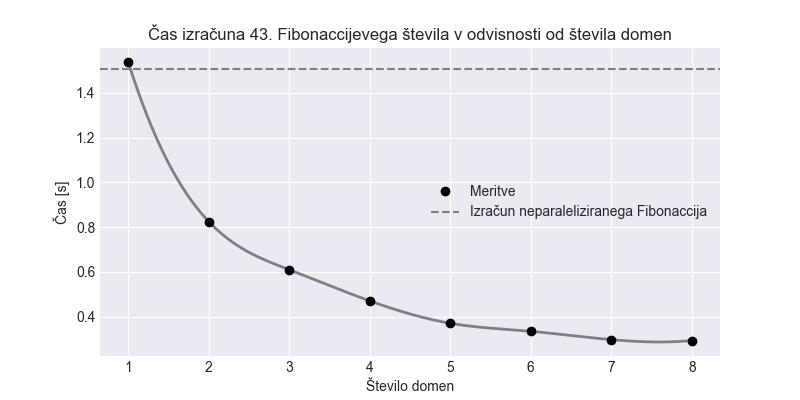
\includegraphics[width=13cm]{slike/fib_par_v_odvisnosti_od_domen.jpg}
  \label{fig:fib_par_v_odvisnosti_od_domen}
\end{figure}

Nadaljnja analiza je bila usmerjena na primerjavo časov izračuna med paralelnim in neparalelnim izvajanjem programa. 
Empirično je bilo ugotovljeno, da neparalelni izračun začne zaostajati pri Fibonaccijevih številih večjih od 38. 
V nasprotju s tem se pri paralelnem izvajanju čas izračuna povečuje manj intenzivno, kot je razvidno iz Slike 
\ref{fig:fib_par_v_odvisnosti_od_n}. Ta razlika potrjuje učinkovitost paralelizacije pri obdelavi večjih nalog.

\begin{figure}[h!]
  \centering
  \caption{Čas izračuna Fibonaccijevih števil v odvisnosti od zahtevanega Fibonaccijevega števila: Paralelno in neparalelno}
  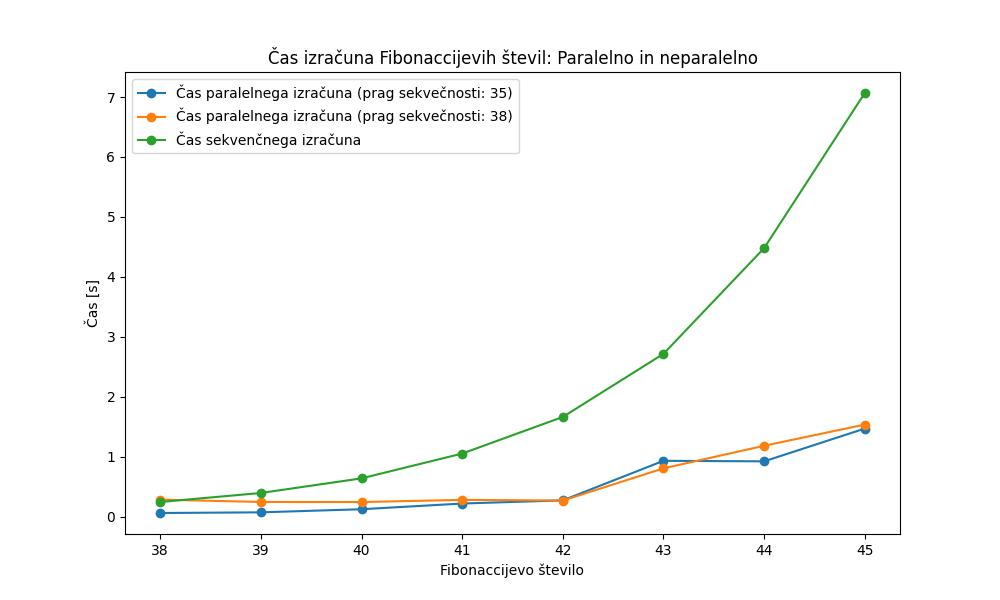
\includegraphics[width=15cm]{slike/fib_par_v_odvisnosti_od_n.jpg}
  \label{fig:fib_par_v_odvisnosti_od_n}
\end{figure}

Zanimivo je tudi opaziti, kako se čas izračuna spreminja pri različnih pragih sekvenčnosti. 
V obravnavanem primeru sta bila uporabljena dva različna praga sekvenčnosti (35 in 38), kar je omogočilo dodatne
vpoglede v učinkovitost in prilagodljivost vzporednega pristopa.

\subsection{Paralelno iskanje v širino (PBFS)}

Breadth-first search (BFS) je algoritem, ki rešuje širok nabor problemov, vključno z raziskovanjem struktur
grafov, iskanjem najkrajših poti v neuteženih grafih, preverjanjem povezanosti med vozlišči ter analizo dvodelnosti grafov.
Dodatno BFS služi kot osnova za naprednejše grafovske algoritme, kot je na primer Dijkstrov algoritem.

Sekvenčna izvedba BFS algoritma temelji na metodologiji upravljanja vrste vozlišč, ki čakajo na raziskavo.
Algoritem izbere in raziskuje vozlišče na čelu vrste, nato pa v vrsto postopoma dodaja njegove neobiskane sosede.
Ta proces se nadaljuje, dokler ni več vozlišč za raziskovanje, kar signalizira zaključek algoritma.
Paralelna različica BFS algoritma predstavlja večji izziv, saj zahteva naprednejšo koordinacijo in upravljanje več
niti izvedbe. Navdih za implementacijo paralelnega BFS smo črpali iz \cite{spaa2010}.

\subsubsection{Sekvenčni BFS}

V kontekstu funkcijskih programskih jezikov, kjer je rekurzija temeljni gradnik, smo k implementaciji BFS algoritma
pristopil rekurzivno. 

Algoritem izvaja iskanje po nivojih, pri čemer sistematično dodaja vsa dosegljiva vozlišča iz trenutnega nivoja v naslednji nivo.
Splošno, za vsako vozlišče $u$ trenutnega nivoja $L$ se v naslednji nivo $L'$ vključijo vsi njegovi sosedi, ki še niso
bili obiskani. 

Ključna metoda v tej implementaciji je \textit{loop}, ki sproži postopek iskanja od začetnega vozlišča, uporabljajoč funkcijo
\textit{mapper} za določanje naslednjega nivoja. Ta funkcija transformira seznam vozlišč trenutnega nivoja v množico
vozlišč naslednjega nivoja, pri čemer se uporablja funkcija \textit{mapper\_seq} za pridobivanje sosednjih vozlišč.
V paralelni verziji algoritma pa bomo uporabili paralelni verzijo funkcije \textit{map} za pridobivanje sosednjih vozlišč.
Metoda \textit{loop} kliče pomožno funkcijo \textit{loop\_inner}. Ta funkcija obravnava trenutni seznam
nivojev (\textit{stages}), pri čemer za vsak nivo identificira vse dosegljive in še neobiskane sosede.
Ti sosedi so nato združeni v naslednji nivo, ki se doda v seznam nivojev. Proces se nadaljuje, dokler ne ostane brez
vozlišč za raziskovanje, kar označuje zaključek BFS.

Metoda \textit{sequential} predstavlja vstopno točko algoritma, ki z uporabo funkcije \textit{mapper\_seq} izvede
sekvenčno verzijo BFS. Ta funkcija deluje tako, da na seznamu trenutnega nivoja za vsako vozlišče poišče sosede znotraj grafa.

Taka implementacija omogoča učinkovito in jasno razumevanje delovanja BFS v funkcijskem programiranju. Prav tako je zaradi
svoje modularne zasnove enostavno razširljiva na paralelno verzijo algoritma.

\begin{lstlisting}[label=lst:bfs_sequential]
module BfsAlgorithms : Bfs = struct
  let loop (start_node : Node.t) 
      (mapper : Node.t list -> NodeSet.t list)
      (graph : UnweightedGraph.t) : NodeSet.t list =
    let rec loop_inner (visited : NodeSet.t) 
        (stages : NodeSet.t list)
        (mapper : Node.t list -> NodeSet.t list) 
        (graph : UnweightedGraph.t) : NodeSet.t list =
      match stages with
      | last_stage :: _ ->
          let all_neighbors =
            last_stage |> NodeSet.elements |> mapper
            |> List.fold_left NodeSet.union NodeSet.empty
          in
          let next =
            NodeSet.diff all_neighbors visited
            |> NodeSet.elements
            |> List.fold_left
                 (fun set node -> NodeSet.add node set)
                 NodeSet.empty
          in
          if NodeSet.is_empty next then List.rev stages
          else
            loop_inner
              (NodeSet.union visited next)
              (next :: stages) mapper graph
      | [] -> failwith "Should not happen"
    in
    let start_visited = NodeSet.singleton start_node in
    loop_inner start_visited [ start_visited ] mapper graph

  let sequential (graph : UnweightedGraph.t) 
      (start_node : Node.t) : NodeSet.t list =
    let mapper_seq : Node.t list -> NodeSet.t list =
     fun nodes ->
      nodes |> List.map (
        fun node -> UnweightedGraph.neighbours node graph)
    in
    loop start_node mapper_seq graph
end
\end{lstlisting}

\subsubsection{Paralelni BFS}

Glavna razlika med sekvenčno in paralelno verzijo algoritma je v tem, da paralelna verzija uporablja paralelno verzijo
funkcije \textit{map} za pridobivanje sosednjih vozlišč. Paralelna verzija funkcije \textit{map} je implementirana
v modulu \texttt{BfsAlgorithms} kot funkcija \texttt{parallel\_map}. Ta funkcija sprejme funkcijo \textit{f}, ki jo
želimo vzporedno izvajati na seznamu elementov, ter seznam elementov, na katerih želimo izvajati funkcijo \textit{f}.
Nato funkcija \texttt{parallel\_map} vzporedno izvede funkcijo \textit{f} na vsakem elementu seznama, ter vrne seznam
rezultatov. Implementacija funkcije \texttt{parallel\_map} je prikazana v \ref{lst:bfs_parallel}.

\begin{lstlisting}[label=lst:bfs_parallel]
module BfsAlgorithms : Bfs = struct
  ...

  let parallel_map (f : 'a -> 'b)
      (task_pool : T.pool)
      (arr : 'a array) : 'b array =
    let len = Array.length arr in
    let res = Array.make len (f arr.(0)) in
    T.parallel_for 
      task_pool 
      ~start:0 
      ~finish:(len - 1) 
      ~body:(fun i ->
        res.(i) <- f arr.(i));
    res

  let parallel (graph : UnweightedGraph.t)
      (start_node : Node.t)
      (task_pool : T.pool) : NodeSet.t list =
    let mapper_par : Node.t list -> NodeSet.t list =
     fun nodes ->
      nodes |> Array.of_list
      |> parallel_map
        (fun node -> UnweightedGraph.neighbours node graph)
        task_pool
      |> Array.to_list
    in
    loop start_node mapper_par graph

  ...
end

\end{lstlisting}

Paralelna izvedba BFS algoritma ključno vključuje uporabo metode \textit{T.run} iz knjižnice Domainslib. Ta metoda je
nujna za obvladovanje notranjih algebraičnih učinkov, ki nastanejo zaradi sinhronizacije nalog med različnimi procesorskimi nitmi.
Ko v paralelni izvedbi uporabimo funkcijo \textit{parallel\_for}, \textit{T.run} zagotavlja, da so vse vzporedno
izvajane naloge pravilno usklajene. Tako poskrbimo za varno izvajanje paralelnih nalog.
Notranji algebraični učinki pri paralelnem izvajanju se nanašajo na procese, ki so potrebni za usklajevanje dostopa do
skupnih podatkovnih struktur in za koordinacijo nadaljevanja obdelave po zaključku posameznih vzporednih nalog.

Za praktičen primer uporabe paralelnega BFS in merjenje časa izvajanja lahko uporabimo naslednji pristop, kot je prikazano v spodnjem izseku kode:

\begin{lstlisting}[label=lst:bfs_calculation_time]
let bfs_par_calculation_time 
    (graph : UnweightedGraph.t) 
    (start_node : Node.t)
    (num_domains : int) : float =
  let task_pool = T.setup_pool ~num_domains () in
  let start_time = Unix.gettimeofday () in
  let _ = T.run task_pool (
    fun () -> Bfs.parallel graph start_node task_pool) in
  let calculation_time =
    Unix.gettimeofday () -. start_time in
  T.teardown_pool task_pool;
  calculation_time
\end{lstlisting}

Ta funkcija ustvari bazen nalog (\textit{task\_pool}) glede na določeno število domen in nato uporabi \textit{T.run} za
izvajanje paralelnega BFS algoritma. Po izvedbi se izmeri časovna razlika, kar nam da čas izračuna algoritma.
Na koncu se bazen nalog razstavi, s čimer se osvobodijo viri, ki so bili uporabljeni za izvajanje algoritma.

\subsubsection{Analiza časa računanja BFS algoritmov}

Analiza časovne učinkovitosti paralelnega algoritma za iskanje v širino (BFS) v primerjavi s sekvenčnim pristopom je
razkrila, da med obema pristopoma ni bistvenih razlik v hitrosti izračuna.
Ta ugotovitev je bila dosežena z izvedbo testov na različno velikih grafih.

Testiranje paralelnega BFS algoritma je bilo izvedeno na grafu z 6000 vozlišči in 1000000 povezavami, pri čemer je
bilo število uporabljenih domen sistematično spreminjano. Izbrana velikost grafa je zagotavljala ravnotežje med
natančnostjo meritev in izogibanjem prekomerni računski obremenitvi. Rezultati testov, prikazani v \ref{fig:bfs_calculation_time_by_num_domains},
ne kažejo jasne korelacije med časom izračuna in številom uporabljenih domen.

\begin{figure}[h!]
  \centering
  \caption{Čas izračuna paralelnega BFS algoritma v odvisnosti od števila domen}
  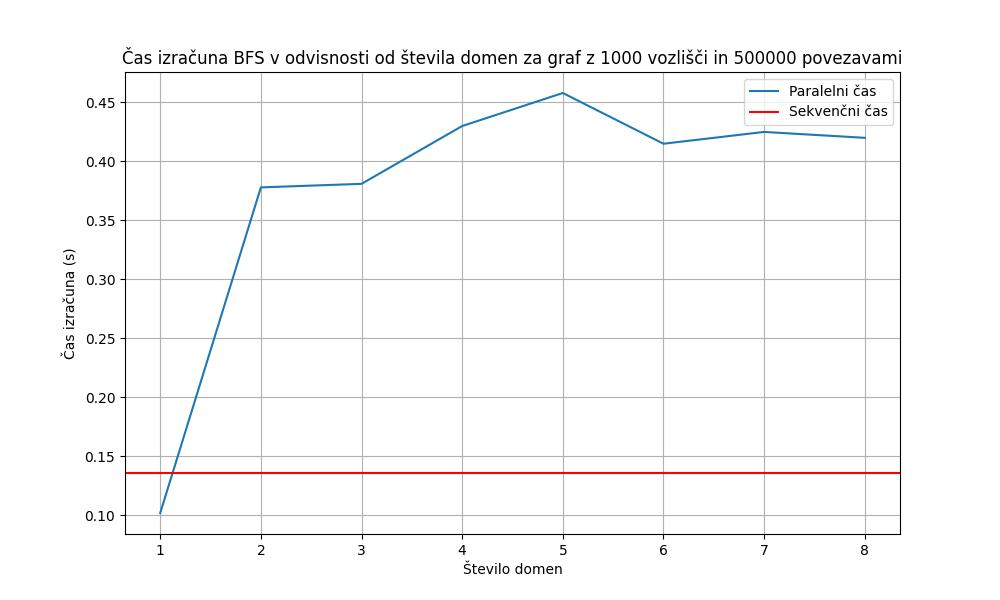
\includegraphics[width=15cm]{slike/bfs_v_odvisnosti_od_stevila_domen.jpg}
  \label{fig:bfs_calculation_time_by_num_domains}
\end{figure}

Poleg tega je bila izvedena primerjava časov izračuna sekvenčne in paralelne izvedbe algoritma na grafih z različnimi velikostmi.
Rezultati so prikazani na \ref{fig:bfs_calculation_time_by_graph_size} in kažejo, da čas izračuna tako za sekvenčni kot za paralelni
pristop linearno narašča s številom vozlišč in povezav v grafu. Vendar pa med časom izračuna sekvenčnega in paralelnega algoritma
ni bilo opaženih bistvenih razlik. Pri analizi je bilo ohranjeno konstantno razmerje med številom povezav v grafu in vsemi
možnimi povezavami, imenovano faktor minimizacije. Podobni rezultati so bili opaženi tudi pri drugih faktorjih minimizacije.

\begin{figure}[h!]
  \centering
  \caption{Čas izračuna BFS algoritma v odvisnosti od števila vozlišč ter povezav}
  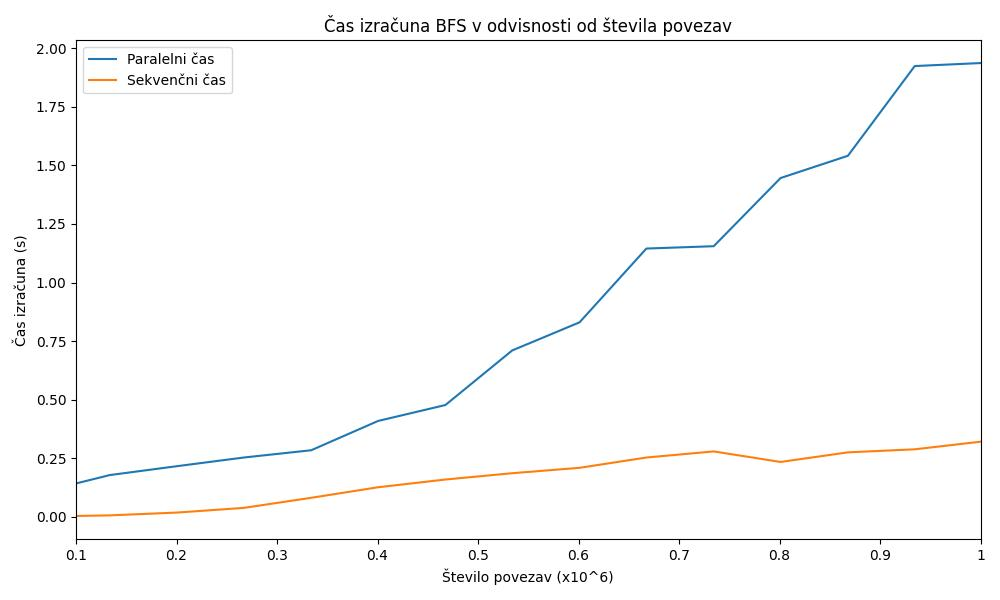
\includegraphics[width=15cm]{slike/bfs_v_odvisnosti_od_velikosti_grafa.jpg}
  \label{fig:bfs_calculation_time_by_graph_size}
\end{figure}

Ti rezultati kažejo, da paralelna implementacija BFS algoritma v nekaterih scenarijih ne prinaša pričakovanih izboljšav v času izračuna.
Podobne ugotovitve so zabeležene tudi v drugih študijah. Na primer, v delu \cite{kuroiwa2020analyzing} avtorji ugotavljajo,
da se pri paralelni implementaciji algoritma lahko pojavijo težave, kot je neenakomerna obremenitev procesorjev, kar
lahko vpliva na celotno učinkovitost. Podobno v študiji \cite{rudolf2019breadth} avtorji opozarjajo na izzive, povezane
s sinhronizacijo in obremenitvijo v paralelnih izvedbah BFS algoritma na večjedrni računalniški arhitekturi.
Ta spoznanja odpirajo potrebo po nadaljnjih raziskavah in optimizaciji, s ciljem izboljšati učinkovitost paralelnih implementacij,
zlasti v primeru posebnih vrst grafov, kjer bi bili paralelni algoritmi lahko hitrejši od sekvenčnih.

\subsection{Paralelni Dijkstrov algoritem} \label{section:dijkstra}

Dijkstrov algoritem, bistven za iskanje najkrajših poti v uteženih grafih, se v svoji paralelni implementaciji sooča s
specifičnimi izzivi, ki presegajo tradicionalni sekvenčni pristop. Temeljna razlika v paralelni različici algoritma,
kot je implementirana v tem delu, leži v paralelnem posodabljanju prioritete vrste z sosedi iz trenutnega vozlišča.
Ta pristop izkorišča več procesorskih jeder za hkratno preverjanje in posodabljanje sosednjih vozlišč, kar omogoča
potencialno skrajšanje časa izračuna pri obsežnih grafih. 

V naslednjem poglavju bomo najprej raziskali funkcijsko implementacijo prioritetne vrste, ki je potrebna za izvajanje
paralelnega Dijkstrovega algoritma. Nato bomo predstavili sekvenčno in paralelno implementacijo Dijkstrovega algoritma. 
Na koncu bomo predstavili analizo časovne učinkovitosti paralelnega Dijkstrovega algoritma.

\subsubsection{Implementacija vrste s prednostjo}

Vrsta s prednostjo igra osrednjo vlogo v Dijkstrovem algoritmu, saj omogoča učinkovit izbor naslednjega vozlišča za raziskovanje. 
Pri tem je pomembno, da je zaradi skupnega pomnilnika vrsta s prednostjo nespremenljiva, saj je v obratnem primeru treba
še skrbeti, da ne pride do konfliktov pri dostopu ter spreminjanju skupnega pomnilnika (ang. thread race). 
Definirali smo modul PQ, kjer je vsak element v kopici je vozlišče s prioritetno vrednostjo ter levim in desnim poddrevesom
(označeno s tipom \texttt{t} v \ref{lst:pq_sig}). Implementacija vrste s prednostjo je povzeta po \cite{okasaki1996}.

\begin{lstlisting}[label=lst:pq_sig]
module PQ : sig
  type t

  exception Queue_is_empty

  val empty : unit -> t
  val is_empty : t -> bool
  val insert : Node.t -> float -> t -> t
  val extract : t -> float * Node.t * t
end = struct
  type t = Empty | PQNode of float * Node.t * t * t

  ...
end
\end{lstlisting}

Glavni operaciji vrste - vstavljanje in izločanje obe sledita istemu principu. Preko ujemanja vzorcev (ang. pattern matching)
primerjamo prioriteto trenutnega korena z vrednostjo, ki jo vstavljamo ali izločamo. V odvisnosti od primerjave trenutne
prioritete z vrednostjo, ki jo vstavljamo ali izločamo, se izvede ustrezna operacija. Za preprečevanje izrojenih dreves
se uporablja rotacija poddreves, kar pomaga ohranjati uravnoteženost. Implementacija funkcije \textit{insert} je prikazana
v \ref{lst:pq_insert}.

\begin{lstlisting}[label=lst:pq_insert]
module PQ : sig
  ...
end = struct
  ...

  let insert new_node new_priority pq : t =
    let rec insert_aux new_node new_priority pq =
      match pq with
      | Empty -> 
          PQNode (new_priority, new_node, Empty, Empty)
      | PQNode ( existing_priority, 
                 existing_node, 
                 left, 
                 right ) ->
          if new_priority <= existing_priority then
            PQNode
              ( new_priority,
                new_node,
                insert_aux existing_node 
                  existing_priority right,
                left )
          else
            PQNode
              ( existing_priority,
                existing_node,
                insert_aux new_node new_priority right,
                left )
    in
    insert_aux new_node new_priority pq
    ...
end
\end{lstlisting}

V najslabšem primeru je časovna zahtevnost $O(n)$. To se bo namreč zgodilo natanko tedaj, ko bomo ob vsakem vstavljanju
vstavili element z največjo prioriteto ter ga nam bo uspelo vstaviti pod list z največjo globino v drevesu (tedaj
rečemo, da je drevo izrojeno). To pa se bo zgodilo redko, saj ob vsakem rekurzivnem klicu premešamo poddrevesa.
Posledično bo verjetnost, da se bo zgodil najslabši primer, zelo majhna.

\subsubsection{Implementacija Dijkstrovega algoritma}

Osnovna zasnova algoritma tako v vzporedni kot v sekvenčni sledi isti logiki. Razlika je le v tem, da se v paralelni
implementaciji naslednja vozlišča pregleduje vzporedno, medtem ko se v sekvenčni implementaciji pregledujejo zaporedno.

\textbf{Osnovna logika: } Algoritem začne z izbiro začetnega vozlišča in inicializacijo vrste s prednostjo, kjer so
vozlišča urejena glede na njihovo razdaljo od začetnega vozlišča. Na vsakem koraku algoritem izvleče vozlišče z najmanjšo
razdaljo od začetnega vozlišča in ga pregleda. Nato se za vsakega soseda tega vozlišča izračuna nova razdalja od začetnega
vozlišča. Ključno vlogo pri zagotavljanju učinkovitosti algoritma igra vrsta s prednostjo, ki omogoča hitro izbiranje
naslednjega vozlišča za obdelavo glede na njegovo razdaljo. Razlika med implementacijama algoritmov se skriva v tem,
kako se izvaja pregledovanje sosedov:

\begin{itemize}
  \item \textbf{Sekvenčna implementacija: } V sekvenčni verziji se vsako posodabljanje razdalj izvaja zaporedno.
    Za vsako izvlečeno vozlišče algoritem preveri vse njegove sosede in posodobi njihove razdalje, če je to potrebno.
    Ta pristop je preprost in učinkovit za manjše ali manj kompleksne grafe.
  \item \textbf{Paralelna implementacija: } Paralelna verzija pri trenutnem vozlišču deli pregledovanje sosedov med
    več procesorskih niti, kjer vsaka nit vzporedno posodablja razdalje sosednjih vozlišč. Za učinkovito vzporedno
    izvajanje tudi tu uporabljam funkcijo \textit{T.parallel\_for} iz knjižnice Domainslib.
\end{itemize}

zaradi bolj natančnih rezultatov testiranja, je bila implementirana verzija Dijkstre, ki se od začetnega vozlišča
razširi do vseh vozlišč v grafu, saj bi pri Dijkstri, ki potuje od začetnega do končnega vozlišča lahko po naključju
hitro prišli do konca grafa, kar bi lahko povzročilo napačne rezultate. Implementacija je priložena v \ref{lst:dijkstra}.

\begin{lstlisting}[label=lst:dijkstra]

module DijkstraAlgorithms : Dijkstra = struct
  let loop (graph : WeightedGraph.t) (start_node : Node.t)
      ~(task_pool_opt : T.pool option) : unit =
    let update_pq pq neighbours
        (current_cost : float) (new_visited : NodeSet.t)
        ~(task_pool_opt : T.pool option) =
      let pq_ref = ref pq in
      let update_queue_for_neighbor (i : int)
          (neighbours_array : (Node.t * float) array) =
        let neighbor, weight = neighbours_array.(i) in
        if not (NodeSet.mem neighbor new_visited) then
          pq_ref := PQ.insert neighbor 
            (current_cost +. weight) !pq_ref
      in
      let neighbours_array = Array.of_list neighbours in
      match task_pool_opt with
      | None ->
          for i = 0 to Array.length neighbours_array - 1 do
            update_queue_for_neighbor i neighbours_array
          done;
          !pq_ref
      | Some task_pool ->
          T.parallel_for task_pool ~start:0
            ~finish:(Array.length neighbours_array - 1)
            ~body:(fun i -> 
              update_queue_for_neighbor i neighbours_array);
          !pq_ref
    in
    let rec loop_inner 
        (pq : PQ.t) (visited : NodeSet.t) : unit =
      if PQ.is_empty pq then ()
      else
        let cost, node, pq = PQ.extract pq in
        let new_visited = NodeSet.add node visited in
        let neighbours =
          graph |> WeightedGraph.edges |> NodeMap.find node
          |> NodeMap.bindings
        in
        let new_pq = update_pq 
          pq neighbours cost new_visited ~task_pool_opt
        in
        loop_inner new_pq new_visited
    in
    let pq_start = 
      PQ.empty () |> PQ.insert start_node 0.0 in
    loop_inner pq_start NodeSet.empty

  let sequential graph start_node =
    loop graph start_node ~task_pool_opt:None

  let parallel graph start_node task_pool =
    loop graph start_node ~task_pool_opt:(Some task_pool)
end
\end{lstlisting}

V Dijkstrovem algoritmu bistveno prispeva k učinkovitosti uporaba nespremenljive vrste s prednostjo, ki omogoča
hitrejše izbiranje naslednjega vozlišča za raziskovanje. To je še posebej pomembno v obsežnih grafih z velikim številom
vozlišč, kjer lahko takšna optimizacija znatno zmanjša skupni čas izračuna. Ključna prednost nespremenljive vrste s
prednostjo v paralelnem kontekstu je v tem, da odpravlja potrebo po sinhronizaciji med večimi procesorskimi nitmi,
s čimer se izognemo težavam, kot je ``dirka podatkov''. To ne samo izboljša varnost in zanesljivost paralelnega izvajanja
algoritma, temveč tudi ohranja visoko učinkovitost paralelne obdelave, kar je ključno za optimizacijo časa izračuna v
kompleksnejših grafovskih strukturah.

\subsubsection{Analiza časa izračuna Dijkstrovega algoritma}

Tokrat je bil za analizo izbran minimizacijski faktor 0.3, kar pomeni, da je število povezav v grafu 30\% od števila vseh
možnih povezav. V analizi smo najprej primerjali čas izračuna Dijkstrovega algoritma v odvisnosti od števila domen,
nato pa še primerjal čas izračuna sekvenčne in paralelne izvedbe algoritma. Rezultati pri drugih minimizacijskih
faktorjih so bili podobni.

Analiza je razkrila, da optimalno število domen za izvajanje paralelnega algoritma ni nujno najvišje možno - najkrajši
čas izračuna smo dobili pri treh domenah. Podoben rezultat je bil opažen tudi pri drugih minimizacijskih faktorjih.
Ta pojav bi lahko razložili z domnevo, da pri večjem številu domen komunikacijski in usklajevalni stroški med domenami
postanejo previsoki, kar lahko pripelje do zmanjšane učinkovitosti. Zato je mogoče, da je optimalno število domen za
izvajanje algoritma manjše, kar se odraža v najkrajšem času izračuna pri treh domenah. 
Rezultati so prikazani na sliki \ref{fig:dijkstra_calculation_time_by_num_domains}.

\begin{figure}[h!]
  \centering
  \caption{Čas izračuna paralelnega Dijkstrovega algoritma v odvisnosti od števila domen}
  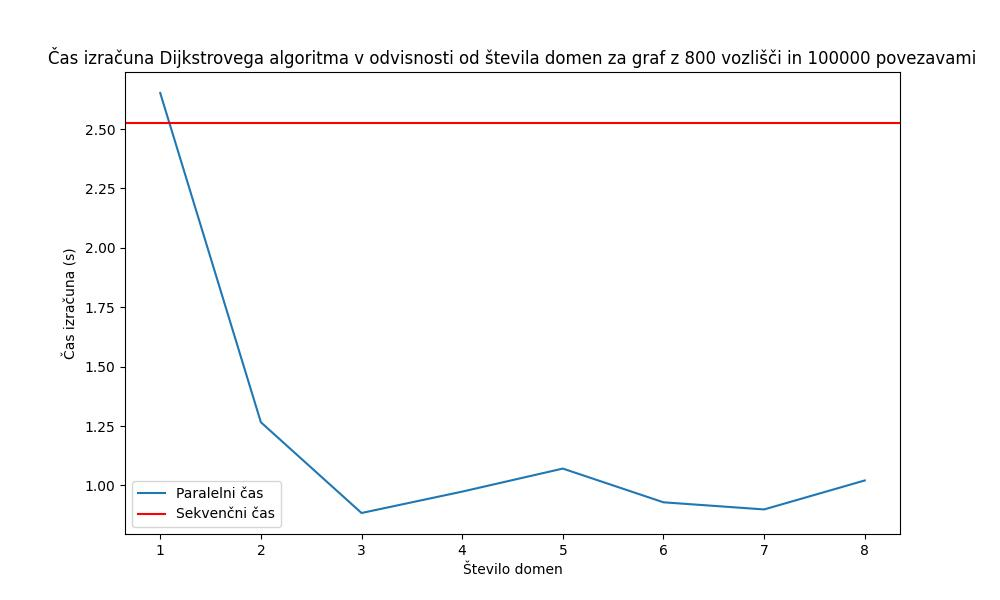
\includegraphics[width=15cm]{slike/dijkstra_v_odvisnosti_od_stevila_domen.jpg}
  \label{fig:dijkstra_calculation_time_by_num_domains}
\end{figure}

Nato smo analizirali še, kako se čas izračuna sekvenčne in paralelne verzije Dijkstrovega algoritma spreminja z rastjo
velikosti grafa. Rezultati, prikazani na sliki \ref{fig:dijkstra_calculation_time_by_graph_size}, kažejo, da čas izračuna
obeh verzij algoritma narašča hitreje kot linearno s številom vozlišč in povezav v grafu, kar je skladno s pričakovanji
za Dijkstrov algoritem. Vidimo, da je paralelni algoritem hitrejši od sekvenčnega. Na primer, pri grafu z 1000 vozlišči
in 150000 je čas izračuna sekvenčnega algoritma približno 3-krat večji kot pri paralelnem algoritmu. Vidimo tudi, da je
na večjih grafih razlika med časom izračuna sekvenčne in paralelne verzije algoritma večja.  

\begin{figure}[h!]
  \centering
  \caption{Primerjava časov izračuna sekvenčne in paralelne implementacije Dijkstrovega algoritma v odvisnosti od velikosti grafa}
  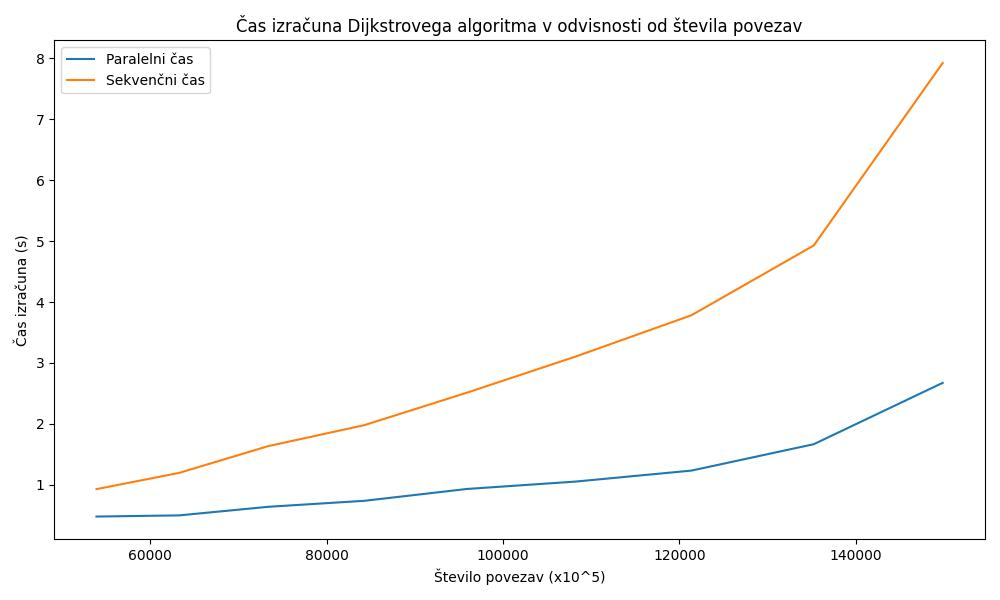
\includegraphics[width=15cm]{slike/dijkstra_v_odvisnosti_od_velikosti_grafa.jpg}
  \label{fig:dijkstra_calculation_time_by_graph_size}
\end{figure}

Naša implementacija je pokazala, da paralelizacija Dijkstrovega algoritma lahko izboljša učinkovitost obdelave velikih
in kompleksnih grafov. Ključnega pomena je najti ravnotežje med številom uporabljenih procesorskih domen in
komunikacijskimi ter usklajevalnimi stroški, ki nastanejo pri paralelnem izvajanju. Optimalno število domen se spreminja
glede na lastnosti grafa, kot so velikost in gostota povezav. Naša analiza podpira ugotovitve Crauserja in
sodelavcev \cite{crauser1998parallelizing}, ki so prav tako uspeli implementirati učinkovito paralelno verzijo Dijkstrovega algoritma.
Ta študija odpira nove možnosti za nadaljnje raziskovanje učinkovitosti paralelizacije v grafovskih algoritmih in
poudarja potrebo po prilagodljivem pristopu za dosego optimalnih rezultatov.

\subsection{Paralelni Floyd-Warshall algoritem}

Floyd-Warshallov algoritem predstavlja klasičen pristop za iskanje najkrajših poti med vsemi pari vozlišč v grafu.
Ta algoritem, ki je bil neodvisno razvit s strani Roberta Floyda in Stephena Warshalla, deluje na principu dinamičnega
programiranja in je zmožen obravnavati grafe z negativnimi težami robov, ob predpostavki, da ne vsebujejo negativnih ciklov.
Algoritem sistematično preučuje vse možne poti med vsakim parom vozlišč in posodablja najkrajšo znano pot, če najde krajšo alternativo.
To doseže z iterativnim pregledovanjem vseh vozlišč in posodabljanjem razdalj med pari vozlišč glede na razdaljo prek vmesnega vozlišča.
Čeprav je njegova časovna zahtevnost $O(n^3)$, kjer n predstavlja število vozlišč v grafu, je še vedno zelo cenjen v situacijah, kjer
je treba pogosto izračunati najkrajše poti med pari vozlišč, na primer v omrežnih analizah in pri načrtovanju logističnih poti.

\subsubsection{Sekvenčna implementacija Floyd-Warshallovega algoritma}

Originalni Floyd-Warshallov algoritem je zasnovan na trikratno gnezdeni zanki \texttt{for}, ki sistematično iterira skozi vse pare vozlišč v grafu.
Vsaka iteracija algoritma posodobi matriko razdalj za vsak par vozlišč, če se najde krajša pot preko predpisanega vmesnega vozlišča.

Implementacija algoritma je preprosta. V \ref{lst:floyd_warshall_seq} je priložena implementacija sekvenčne verzije algoritma, skupaj s pomožno metodo
\texttt{init\_matrix}, ki grafu priredi matriko razdalj. Metoda \texttt{floyd\_warshall\_seq} pa za vsak par vozlišč $(i, j)$
posodobi razdaljo, če obstaja krajša pot prek vmesnega vozlišča $k$.

\begin{lstlisting}[label=lst:floyd_warshall_seq]
module FloydWarshallAlgorithms : FloydWarshall = struct

  let init_matrix graph =
    let nodes = WeightedGraph.nodes graph in
    let n = List.length nodes in
    let matrix = Array.make_matrix n n infinity in
    nodes
    |> List.iter (fun node_from ->
           WeightedGraph.neighbours node_from graph
           |> List.iter (fun (node_to, edge_weight) ->
                  matrix.(Node.id node_from).(Node.id node_to) <- edge_weight));
    matrix |> Array.iteri (fun i row -> row.(i) <- 0.0);
    matrix
  
  let update_distance matrix i j k =
    matrix.(i).(j) <- 
      min matrix.(i).(j) (matrix.(i).(k) +. matrix.(k).(j))

  let floyd_warshall_seq graph =
    let matrix = init_matrix graph in
    let n = Array.length matrix in
    for k = 0 to n - 1 do
      for i = 0 to n - 1 do
        for j = 0 to n - 1 do
          update_distance matrix i j k
        done
      done
    done;
    matrix

end
\end{lstlisting}


\subsubsection{Paralelna implementacija Floyd-Warshallovega algoritma}

V kontekstu paralelizacije nekatere izmed teh zank lahko izvajamo vzporedno, kar lahko zmanjša čas izračuna.

Zunanja zanka \texttt{for k} ne omogoča paralelizacije, saj je posodabljanje najkrajših razdalj odvisno od rezultatov
prejšnjih iteracij. V vsaki iteraciji \texttt{k}, se vozlišče \texttt{k} uporablja kot vmesna točka za posodobitev
razdalj med vsemi pari vozlišč. Zato je treba zunanjo zanko \texttt{for} izvajati zaporedno.
Obratno pa se drugi dve zanki \texttt{for i} ter \texttt{for j} lahko izvajata vzporedno, saj je posodabljanje razdalj med pari vozlišč
neodvisno od posodabljanja drugih parov vozlišč.

Empirično smo poskusili paralelizirati tako zanko \texttt{for i} kot tudi \texttt{for j}, vendar se je izkazalo, da paralelizacija najbolj
notranje zanke \texttt{for j} tvori preveč paralelnih nalog, kar povzroči preveliko komunikacijsko breme in posledično
zmanjšanje učinkovitosti. Najboljše rezultate smo dosegli z vzporedno izvedbo zanke \texttt{for i}.
Implementacija paralelnega algoritma se ne razlikuje precej od sekvenčne verzije. Priložena je v \ref{lst:floyd_warshall_par}.

\begin{lstlisting}[label=lst:floyd_warshall_par]
module FloydWarshallAlgorithms : FloydWarshall = struct
  ...

  let floyd_warshall_par graph pool =
    let matrix = init_matrix graph in
    let n = Array.length matrix in
    for k = 0 to n - 1 do
      T.parallel_for pool 
        ~start:0 
        ~finish:(n - 1) 
        ~body:(fun i ->
          for j = 0 to n - 1 do
            update_distance matrix i j k
          done)
    done;
    matrix

end
\end{lstlisting}

\subsubsection{Analiza časa izračuna Floyd-Warshallovega algoritma}

Analiza časa izračuna Floyd-Warshallovega algoritma se osredotoča na primerjavo med paralelno in sekvenčno izvedbo, hkrati pa razkriva
dinamiko vpliva števila domen na čas izračuna paralelnega algoritma. Iz pridobljenih rezultatov je razvidno, da paralelna implementacija
konsistentno prekaša sekvenčno.

Pri analizi vpliva števila domen na čas izračuna paralelnega algoritma smo opazili zmanjšanje časa izračuna z dodajanjem domen do točke
optimalnega števila, ki je bilo pri šestih domenah. To zmanjšanje časa je verjetno posledica bolj učinkovite porazdelitve izračunov med procesorska jedra,
ki omogoča hitrejšo obdelavo posameznih delov matrike razdalj. Vendar pa po preseganju števila šestih domen opazimo ponovno povečanje časa izračuna.
Ta pojav lahko pripišemo povečanim komunikacijskim in usklajevalnim stroškom, ki nastanejo pri upravljanju večjega števila vzporednih niti.
Ti stroški postopoma zmanjšujejo koristi dodatnih domen, kar vodi v suboptimalno učinkovitost.
Na grafu z 1000 vozlišči smo pognali paralelni algoritem z domenami od 1 do 8. Rezultati so prikazani na sliki \ref{fig:floyd_v_odvisnosti_od_stevila_domen}.


\begin{figure}[h!]
  \centering
  \caption{Čas izračuna paralelnega Floyd-Warshallovega algoritma v odvisnosti od števila domen}
  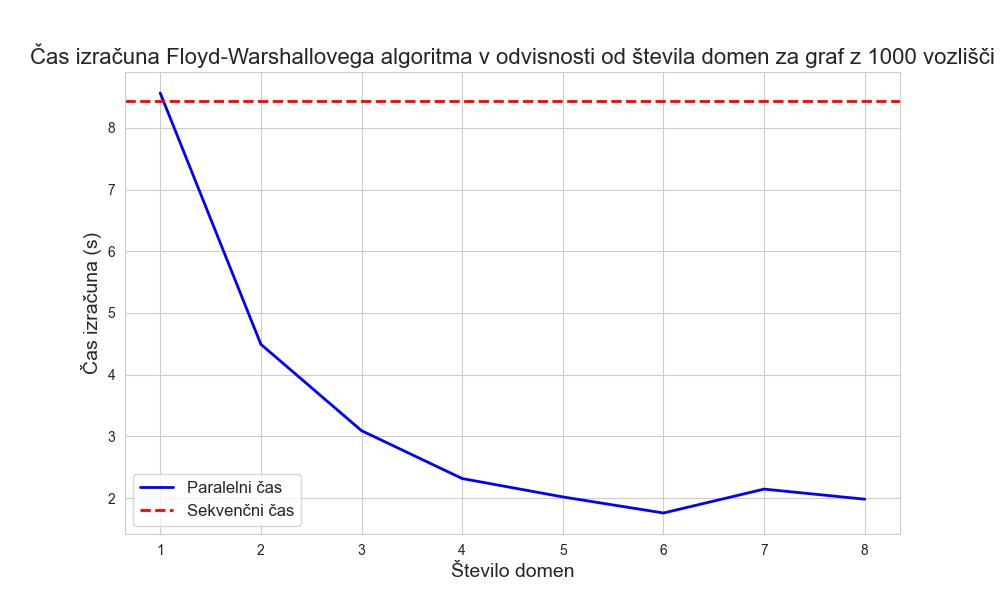
\includegraphics[width=15cm]{slike/floyd_v_odvisnosti_od_stevila_domen.jpg}
  \label{fig:floyd_v_odvisnosti_od_stevila_domen}
\end{figure}

Kar zadeva primerjavo med sekvenčno in paralelno verzijo algoritma, je bilo ugotovljeno, da je sekvenčna verzija približno 4-krat počasnejša
od optimizirane paralelne verzije na grafih z različnimi velikostmi. Rezultati so prikazani na sliki \ref{fig:floyd_v_odvisnosti_od_velikosti_grafa}.

\begin{figure}[h!]
  \centering
  \caption{Primerjava časov izračuna sekvenčne in paralelne implementacije Floyd-Warshallovega algoritma v odvisnosti od števila vozlišč}
  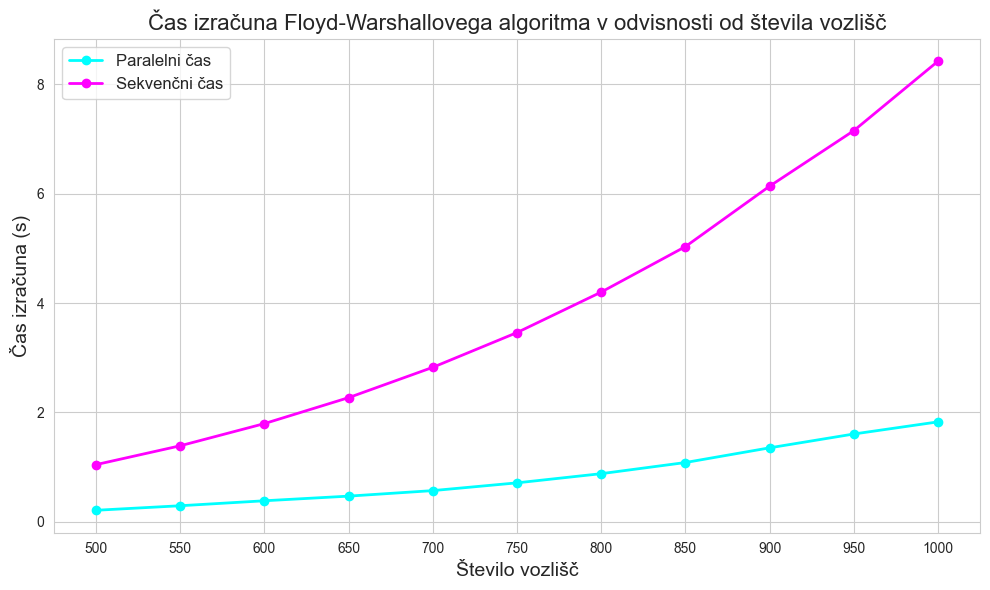
\includegraphics[width=15cm]{slike/floyd_v_odvisnosti_od_velikosti_grafa.jpg}
  \label{fig:floyd_v_odvisnosti_od_velikosti_grafa}
\end{figure}

Zanimivo je, da optimizacija, kjer paraleliziramo obe notranji zanki (\texttt{for i} in \texttt{for j}), ni prinesla pričakovanih izboljšav.
Nasprotno, ta pristop je povzročil povečanje časovnega bremena zaradi komunikacijskih stroškov, kar je privedlo do slabših rezultatov
kot pri sekvenčni izvedbi.

\subsubsection{Zaključek in Alternativni Pristopi za Floyd-Warshallov Algoritem}

Čeprav se je v naši analizi paralelna implementacija Floyd-Warshallovega algoritma izkazala za učinkovitejšo od sekvenčne, obstajajo tudi
alternativne metode, kot je 2D block mapping algoritem \cite{parallel_floyd_warshall}, ki obetajo nadaljnje optimizacije. Ta pristop, ki deli
matriko na manjše bloke za vzporedno obdelavo, lahko potencialno zmanjša komunikacijske stroške in izboljša ravnovesje obremenitve med
procesorskimi jedri. Takšne inovativne strategije odpirajo nove možnosti za izboljšanje paralelnih algoritmov v teoriji grafov,
kar obeta zanimive smeri za prihodnje raziskave.

\section{Zaključek}

V diplomski nalogi smo se osredotočili na problematiko paralelizacije grafovskih algoritmov v funkcijskih programskih jezikih.
Osrednji del naloge je predstavljala implementacija in analiza paralelnih verzij klasičnih grafovskih algoritmov, kot so iskanje v širino (BFS),
Dijkstrov algoritem in Floyd-Warshallov algoritem, v programskem jeziku OCaml z uporabo knjižnice Domainslib. Pomemben del raziskave je
bil posvečen tudi predstavitvi grafa v funkcijskih jezikih, kjer smo razvili nespremenljive podatkovne strukture za učinkovito upravljanje z grafi.

V procesu raziskovanja smo izvedli temeljito analizo časovne učinkovitosti posameznih algoritmov, pri čemer smo primerjali paralelne in sekvenčne izvedbe.
Pri Dijkstrovem ter Floyd-Warshallovem algoritmu so rezultati pokazali izboljšanje učinkovitosti paralelnih verzij, medtem ko je pri paralelnem BFS algoritmu
izboljšave zaradi paralelizacije ni bilo. Odkrili smo tudi, da je optimalno število domen za izvajanje paralelnih algoritmov odvisno od narave problema
in strukture grafa.

Za nadaljnje raziskave smo izpostavili potencial uporabe alternativnih pristopov, kot je 2D block mapping, ki obljubljajo nadaljnje
optimizacije paralelnih algoritmov. Ta diplomska naloga tako prispeva k boljšemu razumevanju in izboljšanju paralelne obdelave grafovskih
algoritmov v funkcijskih jezikih, kar odpira nove možnosti za njihovo uporabo v kompleksnih računalniških problemih.
Hkrati pa moramo upoštevati, da so bile naše ugotovitve dosežene v specifičnih eksperimentalnih okoliščinah, kar pomeni, da bi v drugačnih
kontekstih lahko dosegli drugačne rezultate. To poudarja potrebo po nadaljnjem testiranju in prilagajanju algoritmov za specifične uporabe.

Zaključujemo, da je paralelizacija grafovskih algoritmov v funkcijskih jezikih obetavno področje, ki nudi številne možnosti za raziskovanje in
praktično uporabo, še posebej v obsežnih računalniških sistemih in aplikacijah, ki zahtevajo visoko računsko zmogljivost.
Pokazali smo, da je paralelizacija grafovskih algoritmov v funkcijskih jezikih lahko tudi dobra alternativa paralelizaciji grafovskih algoritmov
v imperativnih programskih jezikih.


\end{document}
